\section{Gearing}\label{robot:gearing}
I \cref{sensorer:motorer} fandt vi ud af at præcisionen på motorerne ikke var høj.
Der var en afvigelse på op til 4\dg, imod en forventet afvigelse på max. 1\dg.

\subsection{Gearing af motorer}
For at sænke denne upræcision vil der blive indført gearing.
Dette er især vigtigt for den motor der roterer den ultrasoniske sensor, men også for de motorer som driver hjulene.

\paragraph{Den ultrasoniske sensor} bruges til at bestemme tilkendegivelse og afstand af et objekt i en bestemt retning, derfor vil det være en klar fordel jo højere sikkerhed og præcision der kan opnås når denne retning skal bestemmes.
Rotationen vil naturligvis foregå langsommere end uden gearing, men tid er ikke en faktor på nuværende tidspunkt.

\paragraph{Hjulene} har vist problemer med at holde fat i underlaget, derfor vil det være en fordel at geare så der kan opnås et højere moment.
Igen er tid ikke en faktor, så det er acceptabelt at robotten mister fart.
Præcision af motorernes position er heller ikke vigtig, da lokationen bestemmes andetsteds og ikke vha. \textit{dead reckoning}.

\subsection{Simpel Teori}\label{gearing:simpel_teori}
Gearing kan foregå på to måder; geare op eller geare ned.
Det tandhjul der er knyttet direkte til motoren kalder vi fører-tandhjulet og det tandhjul der er knyttet til fører-tandhjulet kalder vi for følger-tandhjulet (se evt. \cref{gearing:nedgearing}).

\subsubsection{Nedgearing}
Nedgearing foregår ved at et mindre tandhjul driver et større tandhjul.
Ratio'en (størrelsen af gearing) er styret af antallet af tænder på tandhjulene.
For eksempel vil et 24-tands fører-tandhjul drive et 40-tands følger-tandhjul med ratio'en $\frac{40}{24}$, hvilket betyder at der går 40 fører omdrejninger pr. 24 følger omdrejninger. Dvs. at motoren der driver fører-tandhjulet skal rotere $\frac{40}{24} = \frac{1 \frac{2}{3}}{1}$ omgange for at rotere følger-tandhjulet én omgang.

\begin{figure}[h]
\centering

\includegraphics[width=.5\textwidth]{gears/op_og_ned}
\caption{Eksempel på (ned-)gearing}
\label{gearing:nedgearing}
\end{figure}

\subsection{Vores gearing}
Her vil blive forklaret den teoretiske gearing for henholdsvis ultrasonisk sensor og hjul.

\subsubsection{Ultrasonisk sensor}
Gearingen for den ultrasoniske sensor består af i alt 4 tandhjul, som alle kan ses i \cref{gearing:tandhjul}.

\begin{figure}[h] % De anvendte tandhjul
\centering
\begin{subfigure}[b]{.19\textwidth}
\centering
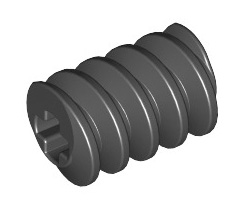
\includegraphics[width=\textwidth]{gears/worm}
\caption{Orm}
\label{gearing:orm}
\end{subfigure}
\begin{subfigure}[b]{.19\textwidth}
\centering

\includegraphics[width=\textwidth]{gears/16-tooth}
\caption{16-tands}
\label{gearing:16tand}
\end{subfigure}
\begin{subfigure}[b]{.19\textwidth}
\centering

\includegraphics[width=\textwidth]{gears/24-tooth}
\caption{24-tands}
\label{gearing:24tand}
\end{subfigure}
\begin{subfigure}[b]{.19\textwidth}
\centering
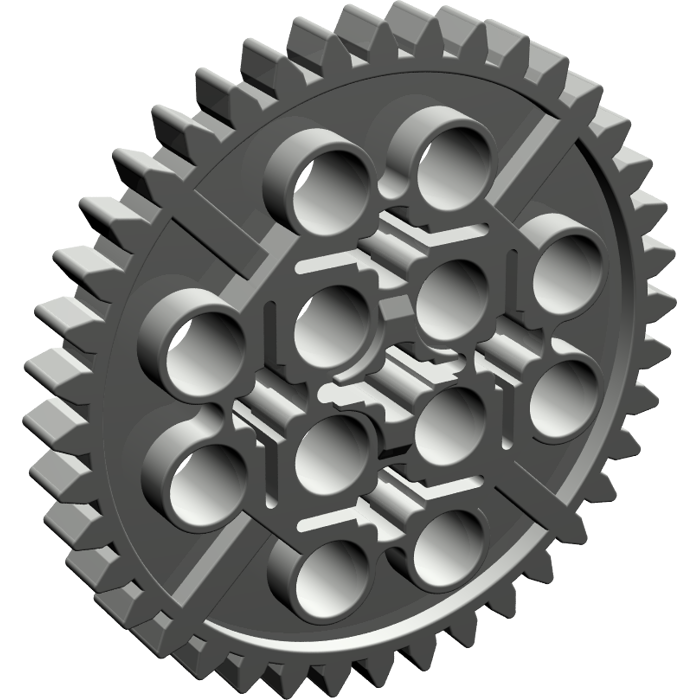
\includegraphics[width=\textwidth]{gears/40-tooth}
\caption{40-tands}
\label{gearing:40tand}
\end{subfigure}
\begin{subfigure}[b]{.19\textwidth}
\centering
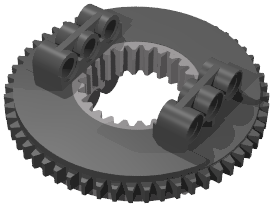
\includegraphics[width=\textwidth]{gears/turntable}
\caption{56-tands \\ \centering (drejeskive)}
\label{gearing:56tand}
\end{subfigure}
\caption{De anvendte tandhjul}
\label{gearing:tandhjul}
\end{figure}

Den første kombination består af en orm (se \cref{gearing:orm}) som fører-gear og 40-tands (se \cref{gearing:40tand}) som følger-gear.
Ormen kræver en hel rotation for at flytte én tand.
Dette giver ratio'en $\frac{40}{1} = 40$, dvs. at der kræves 40 hele motor-rotationer for at rotere 40-tands tandhjulet én omgang.

Den anden kombination består af en 24-tands (se \cref{gearing:24tand}) som fører-tandhjul og en 56-tands (se \cref{gearing:56tand}) som følger-tandhjul.
Dette giver ratio'en $\frac{56}{24} = \frac{2\frac{1}{3}}{1}$.

Den samlede gearing er således: $$\frac{40}{1} \cdot \frac{2\frac{1}{3}}{1} = \frac{93 \frac{1}{3}}{1}$$

\subsubsection{Hjul}
Gearingen for hjulene består hver især af to tandhjul; ét 40-tands og ét 24-tands.
Derved er gearingen som i eksemplet i \cref{gearing:simpel_teori}: $$ \frac{40}{24} = 1 \frac{2}{3} $$

\subsection{Test af gearing}
Nu hvor den teoretiske gearing er fastlagt, vil der her blive udført forsøg for at afgøre præcisionen af motorerne med gearing, evt. at fastlægge en faktisk gearing, hvis denne afviger fra den teoretiske.

\subsubsection{Hjul}
Da præcisionen på hjulene ikke er så vigtig, da der bruges alternativ metode til lokation (og ikke dead reckoning), er der ikke lavet en grundig test.
Der blev udført handlinger med antal hjul-omdrejninger (og ikke motor-omdrejninger) som input, med en beregning fra hjul-omdrejninger til motor-omdrejninger, ud fra den teoretiske gearing.

Der er blevet udført test af henholdsvis; $\frac{1}{8}$, $\frac{1}{4}$, $\frac{1}{2}$, 1, 2, 3, 10 hele hjul-omdregninger.

\paragraph{Resultatet} af testen var positiv.
Samtlige tests gave ingen afvigelse.
Dette resultat, samt vigtigheden, ledte til at der ikke var behov for flere tests af hjul-gearingen.

\subsubsection{Sensor}
Denne test er meget vigtigere end hjul-testen, da det er vigtigt at vide den nøjagtige nuværende rotation af sensoren, for at få så præcis en målings-retning som muligt.

\paragraph{Første test} var en grovtest, hvor der blev kørt i den samme retning i et antal sensor-omdrejninger.
Igen blev der udført handling med sensor-omdrejninger som input, ud fra en beregnet motor-omdrejning, baseret på den teoretiske gearing.
Denne test gav et godt resultat, uden afvigelse.

\paragraph{Anden test} blev udført ved at køre mindre omdrejninger, skiftevis med og mod uret.
Dette gav en upræcision, da der er slør i den øverste gearing, mellem 56-tands og 24-tands tandhjulene.
Dette slør giver mellem $\frac{1}{4}$ og $\frac{3}{4}$ tands unøjagtighed, da der ved skift af rotations-retning bruges op til $\frac{3}{4}$ tandhjul-omdrejning for 24-tands tandhjulet at få fat i 56-tands tandhjulets tænder igen.

\paragraph{Sløret} giver giver en unøjagtighed på mellem $\frac{1}{4}$ og $\frac{3}{4}$ tand.
Dette gør at der kræves ekstra motor-omdrejninger når der skiftes retning.
For den minimale afvigelse skal der bruges: $ \frac{\frac{1}{40}}{\frac{1}{24}}\cdot\frac{1}{4} = 0.15$ ekstra motor-omdrejninger.
For den maksimale afvigelse: $ \frac{\frac{1}{40}}{\frac{1}{24}}\cdot\frac{3}{4} = 0.45$.

Da hver motor-omdrejning svarer til $\frac{1}{93.\overline{3}}$ sensor-omdrejning, giver det at én motor-omdrejning får sensoren til at rotere $\frac{360}{93.\overline{3}} = 3\frac{6}{7}\dg$.
Derved giver dette en afvigelse på minimum $3\frac{6}{7}\cdot0.15 = 0.57\overline{857142}\dg$ og maximum $3\frac{6}{7}\cdot0.45 = 1.73\overline{571428}\dg$.

\paragraph{Optimering af slør} kunne foregå ved altid at køre $0.45 - 0.15 = 0.15$ motor-omdrejninger ekstra, når der skiftes retning.
På denne måde vil den maksimale og ca. afvigelse være $0.57\overline{857142}\dg$.

\begin{figure}[h]
\centering
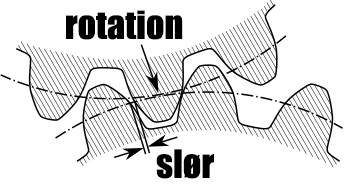
\includegraphics[width=0.5\textwidth]{gears/sloer}
\caption{Slør mellem gear}
\label{gearing:sloer}
\end{figure}